%\section{old Concept}
\subsection{Basic Concept}
Feet are used in many real world tasks together with the rest of the body, but in computer environments they are almost completely put aside as an interaction possibility \cite{pakkanen}. For instance, Ubicomp researches have developed different types of interfaces for public spaces where users' hands are the protagonists and feet are partly or completely neglected. 

The basic concept of this project is a feet-based interface whose \textbf{individual modules} react when pushed or kicked. For this purpose, modules have to be highly \textbf {mobile} to yield a flexible interaction with the user. Another desired aspect is \textbf {expandability}: the envisioned system will allow the integration of new modules and features. Finally, a module is expected to detect if a another module comes up against it. In other words, another feature in the envisioned system is the \textbf{interaction between modules}. 

\subsection{Hardware Concept}
To achieve \textbf{modularity} and \textbf{mobility}, a wireless communication platform is fundamental.   
Panstamps \cite{panstamp} are small boards intended for implementing custom wireless networks. In their boards, Panstamps have an integrated transceiver, the CC1101 \cite{cc1101}, that makes the wireless communication possible. 

Due to Panstamps' open source nature, documentation and information about already implemented projects with them is at hand for everyone on the internet; this represents a very important advantage over other wireless products in the market. Furthermore, Panstamps' core is the the ATMEGA 328 \cite{atmega328}; therefore, they are entirely programmable from the Arduino IDE, whose community is increasing each day.

For all these reasons, our envisioned system is based on Panstamps. As depicted in Figure~\ref{fig:server-module}, each module in our system is constituted by a sensor and actuator node, both having a Panstamp as their nucleus. The server node has also a Panstamp as its main component, which communicates wirelessly with the other modules' panstamps. 

The Java Server gets the data recollected by the server node, process it and gives a response to the server node that has to be sent to the appropriate node in the network. The feedback provided by the Java Server depends entirely on the \emph{personality} of each device.

\begin{figure}[h!]
 \centering
 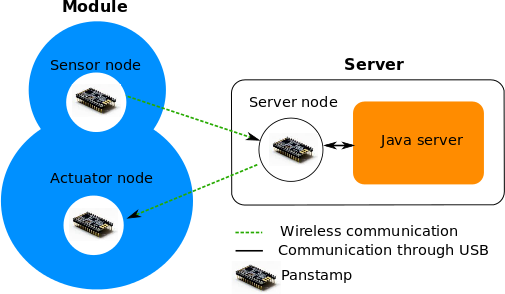
\includegraphics[width= 0.4\textwidth, clip=true  ,keepaspectratio=true]{./graph/entity_server.png}
 \caption{Interface's server and a module}
 \label{fig:server-module}
\end{figure}

To detect if they have been kicked or pushed, modules need to sense their own movement; therefore, an accelerometer is connected to the sensor node of each module as shown by Figure \ref{fig:sensor-node}. We used the ADXL335 \cite{ADXL335}, a small accelerometer that measures acceleration in each of the cardinal directions (x,y and z).

Each module has a led strand constituted by led-and-controller pairs. To produce a certain light pattern, the actuator node, which is connected to the strand (see Figure \ref{fig:actuator-node}), sends information to each controller to indicate whether its led should be on or off and what color has to be displayed. Led patterns play an important role in the interface because each module expresses its \textbf{personality} through led patterns.  

The \textbf{interaction between modules} is based on proximity; that is, a module triggers a reaction in other module when it is close to it. In our implementation, the closeness between two modules is determined by measuring the RSSI of broadcasted messages in the network. The RSSI is a measurement of the power present in a received radio signal. The longer the distance travelled by a radio wave the bigger its intensity loss.

All the elements in a module are powered by a 11 volts Li-Po battery. This battery should not be over-discharged, for this reduces drastically it's life. Therefore, sensor nodes have an integrated voltage-monitoring circuit (see Figure \ref{fig:sensor-node}) that detects the  low-battery state.

\begin{figure}[h!]
 \centering
 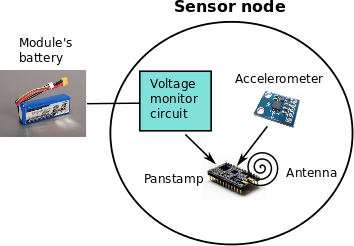
\includegraphics[width= 0.4\textwidth, clip=true  ,keepaspectratio=true]{./graph/sensor_node.png}
 \caption{Sensor node elements}
 \label{fig:sensor-node}
\end{figure}


\begin{figure}[h!]
 \centering
 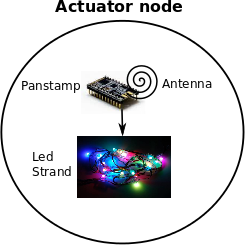
\includegraphics[width= 0.3\textwidth, clip=true  ,keepaspectratio=true]{./graph/actuator_node.png}
 \caption{Actuator node elements}
 \label{fig:actuator-node}
\end{figure}


\subsection{Software Concept} 

\subsubsection{Driver} 
Since we used the Arduino IDE to program the Panstamps, all the nodes' drivers in the network were written in C++. These drivers were designed to allow \textbf{expandability}; as a result, new nodes can be added to the network by coping the basic drivers and changing them slightly. 

In short, the drivers are in charge of:
\begin{itemize}
\item enabling the wireless communication
\item managing the communication between different nodes
\item handling the information provided by sensors 
\item operating the led strands
\item setting up the communication with the Java Server on the Panstamp' side
\end{itemize}

\subsubsection{Java server}

The Java Server is the heart of the interface; it is the orchestrator of all nodes in the system's network. The server node transfers all the data gathered in the network to the Java Server, which produces a response according to each module's personality and sends it to the intended actuator nodes through the server node (See Figure~\ref{fig:server-module}).  



The kinetic inputs "first contact", "played" and "played hard" are triggered by each other:
So when the device gets kicked, his state will change from "standby" to "first contact", then when the threshold is high enough, the state changes directly to "played". There cannot be a change from "first contact" to "played hard". 

Those data will be send to the panstamp of the server where this data will be analyzed and compared to the corresponding personality of the device. The personality then outputs the behaviour for the device. A behaviour consists two colors (which can be the same) and a pattern. This pattern describes the appearance of the colors. (Like a blinking or fading of the LEDs)
The idea was to create typical characters for the devices. Below you can see the table which describes how a device reacts to kinetic inputs into his environment. So if it is in his default state the device "Paul" is fading blue. By changing input the state will change perhaps to the state "hard played". Those behaviour can be manipulated using the servers graphical interface. 


So by using this technique the following rules shown in this table can be implemented.
When the servers got from the device panstamp the data with which other device it is confronted, the server looks up in the data of the presetpersonalities.java file and returns the matching pattern. For this use it is necessary to define which personality is more dominant than another.


So when the server has received the data of its state and his neighbourhood of the sending device it will send a new pattern for the LEDs chain actuator when the situation of the sending device has changed.
When the device hadn't send its data packet for two minutes a warning will pop up in the graphical interface. Apparently this will happen when the device is out of range of the sending area of the panstamp antennas (approximately ~50 metres).
This very functionality is illustrated in the following graphic.



